\dut \ перед началом заряда должен быть разряжен при нормальной температуре окружающей среды током разряда \current \ до конечного напряжения~$21$~В.


\dut \ должен быть заряжен при нормальной температуре окружающей среды следующим образом:
%
\begin{enumerate}
	\item постоянным током~$20$~А до достижения напряжения на источнике тока~$29$~В;
	\item постоянным напряжением~$28,8$~В до падения тока заряда до~$0,4$~А.
\end{enumerate}

Схема заряда \dut \ представлена на рисунке~\ref{fig:charge}.

\begin{figure}[!htb]
	\centering
	\includegraphics[page=3]{schema}
	\begin{picdescription}
		\item \ESKDtheTitle \ \RN;
		\item\label{d:charger} \hyperref[e:charger]{Зарядное устройство \chargerRN};
	\end{picdescription}
	\begin{picdescription}[label={E\arabic* ---}, ref={E\arabic*}, before={\vspace{0pt}\small}]
		\item\label{d:charge} \hyperref[e:charge]{Жгут \chargeRN}.
	\end{picdescription}
	\caption{Схема заряда \dut }
	\label{fig:charge}
\end{figure}

Приблизительное время заряда "--- $2,5$~ч.